\documentclass[aspectratio=1610,usenames,dvipsnames]{beamer}
%
% Choose how your presentation looks.
%
% For more themes, color themes and font themes, see:
% http://deic.uab.es/~iblanes/beamer_gallery/index_by_theme.html
%

\usetheme{Cesbio}      % or try Darmstadt, Madrid, Warsaw, ...
\usecolortheme{default} % or try albatross, beaver, crane, ...
\usefonttheme{default}  % or try serif, structurebold, ...
\setbeamertemplate{navigation symbols}{}
% \setbeamertemplate{footline}[frame number]
\setbeamertemplate{caption}[numbered]

\usepackage[english]{babel}
\usepackage[utf8x]{inputenc}
\usepackage[T1]{fontenc}
\usepackage{multirow}
\usepackage{graphicx}
\usepackage{FiraSans}
\usepackage{grffile}
\usepackage{algorithm2e}
\usepackage{minted}
\usepackage[dvipsnames]{xcolor}

\AtBeginSection[]{
  \begin{frame}
  \vfill
  \centering
  \begin{beamercolorbox}[sep=8pt,center,shadow=true,rounded=true]{title}
    \usebeamerfont{title}\insertsectionhead\par%
  \end{beamercolorbox}
  \vfill
  \end{frame}
}


\bibliographystyle{unsrt}
\title{Avancement thèse MAESTRIA WP2}
\newcommand{\shorttitle}{Avancement WP2 - 12/2020}
\newcommand{\shortauthor}{E. Giry-Fouquet} % Name to display in the footline
\subtitle{Novembre - Décembre 2019}
\author{Erwan GIRY-FOUQUET}
\institute{CESBIO, Toulouse}
\date{18/12/2019}

\begin{document}
{
\setbeamertemplate{footline}{} % Remove footline in titlepage
\begin{frame}
\vspace{.8cm}

\includegraphics[width=1.5cm]{logo_cesbio_transp.pdf}
\titlepage % Print the title page as the first slide
\end{frame}
}

% Uncomment these lines for an automatically generated outline.
%\begin{frame}{Outline}
%  \tableofcontents
%\end{frame}

\section*{Summary}
\begin{frame}
  \tableofcontents
\end{frame}  

\section{Model}

\begin{frame}{Semi-supervisé : log-vraissemblance (1/2)}
    Let us now suppose that, in addition to \(n_l\) labeled training samples \(\big\{\mathbf{x}_{l_l},   z_{l_l}\big\}_{l_l=1}^{n_l}\) , we have access to \(n_u\) unlabeled samples \(\big\{\mathbf{x}_{l_u}\big\}_{l_u=1}^{n_u}\). The complete likelihood can be written as
    % TODO : Mettre ça en bullet points

    \begin{eqnarray*}
      L(\mathbf{X}_l, \mathbf{z}_l, \mathbf{X}_u, \hat{\mathbf{z}}_u, \mathbf{r}) &=& \prod_{l_l=1}^{n_l}
      p(\mathbf{X}=\mathbf{x}_{l_l}, Z=z_{l_l}) 
      \color{Mahogany}{
      \prod_{l_u=1}^{n_u} p(\mathbf{X}=\mathbf{x}_{l_u}, Z=\hat{z}_{l_u})
      }\\
    \end{eqnarray*}
    
    
    where \(\hat{z}_{l_u}\) is some estimation of the class membership.

\end{frame}

% TODO : rajouter frame 
% schéma, en liant les couleurs du précédent slide aux groupes supervisés / non supervisés

\begin{frame}{Semi-supervisé : log-vraissemblance (2/2)}


    Many variants are considered :
    \begin{itemize}
        \item Training set's labels can be fixed or not
        \item Des poids peuvent être utilisés pour ajuster l'influence du jeu de données non labellisé.
    \end{itemize}
    \small
    \begin{eqnarray}
      \label{eq:ll:ss}
          \begin{array}{rl}
            \displaystyle{\min_{\mathbf{r}}}
            
            &\displaystyle{
            
                \frac{1}{n_l}\sum_{i=1}^C \sum_{\substack{l_s=1\\ z_l \in i}}^{n_i}  -\ln\big(\mathbf{r}_i^\top \boldsymbol{\psi}_{l_s}\big)
            
                + \color{Mahogany}{
                    \frac{1}{n_u}  \sum_{l_u=1}^{n_u} - \ln\big(\sum_{i=1}^C \hat{z}_{l_ui} \mathbf{r}_i^\top \boldsymbol{\psi}_{l_u}\big)
                }
            
            }\\
            
               \text{Constraint to} & \mathbf{A}\mathbf{r} = \mathbf{1}\\
              & \mathbf{r} \succcurlyeq 0
          \end{array}
     \end{eqnarray}
     \normalsize

\end{frame}

\begin{frame}{Semi-supervisé : algorithme EM}

    
    \begin{algorithm}[H]
        \SetAlgoLined
        \KwResult{\(\hat{\mathbf{r}}, \hat{\mathbf{z}}\)}
        Run ADDM on the labeled set only to get \(\mathbf{r}^{0}\)\;
         \While{\(L^{(t)}\) is increased and $t < t_{max}$}{
           \textbf{E-Step}: Estimate \(\textbf{z}_{l_u}^{(t)}\) using mixture model\;
           \textbf{M-Step}: Maximize \(L^{(t)}\) w.r.t. to \(\textbf{r}^{(t)}\)\;
         }
         \caption{Semi-supervised algorithm}
         \label{algo:em}
    \end{algorithm}
\end{frame}


\section{Code}

\begin{frame}{Profiling}



\begin{columns}
    \begin{column}{0.49\textwidth}
        \begin{center}
            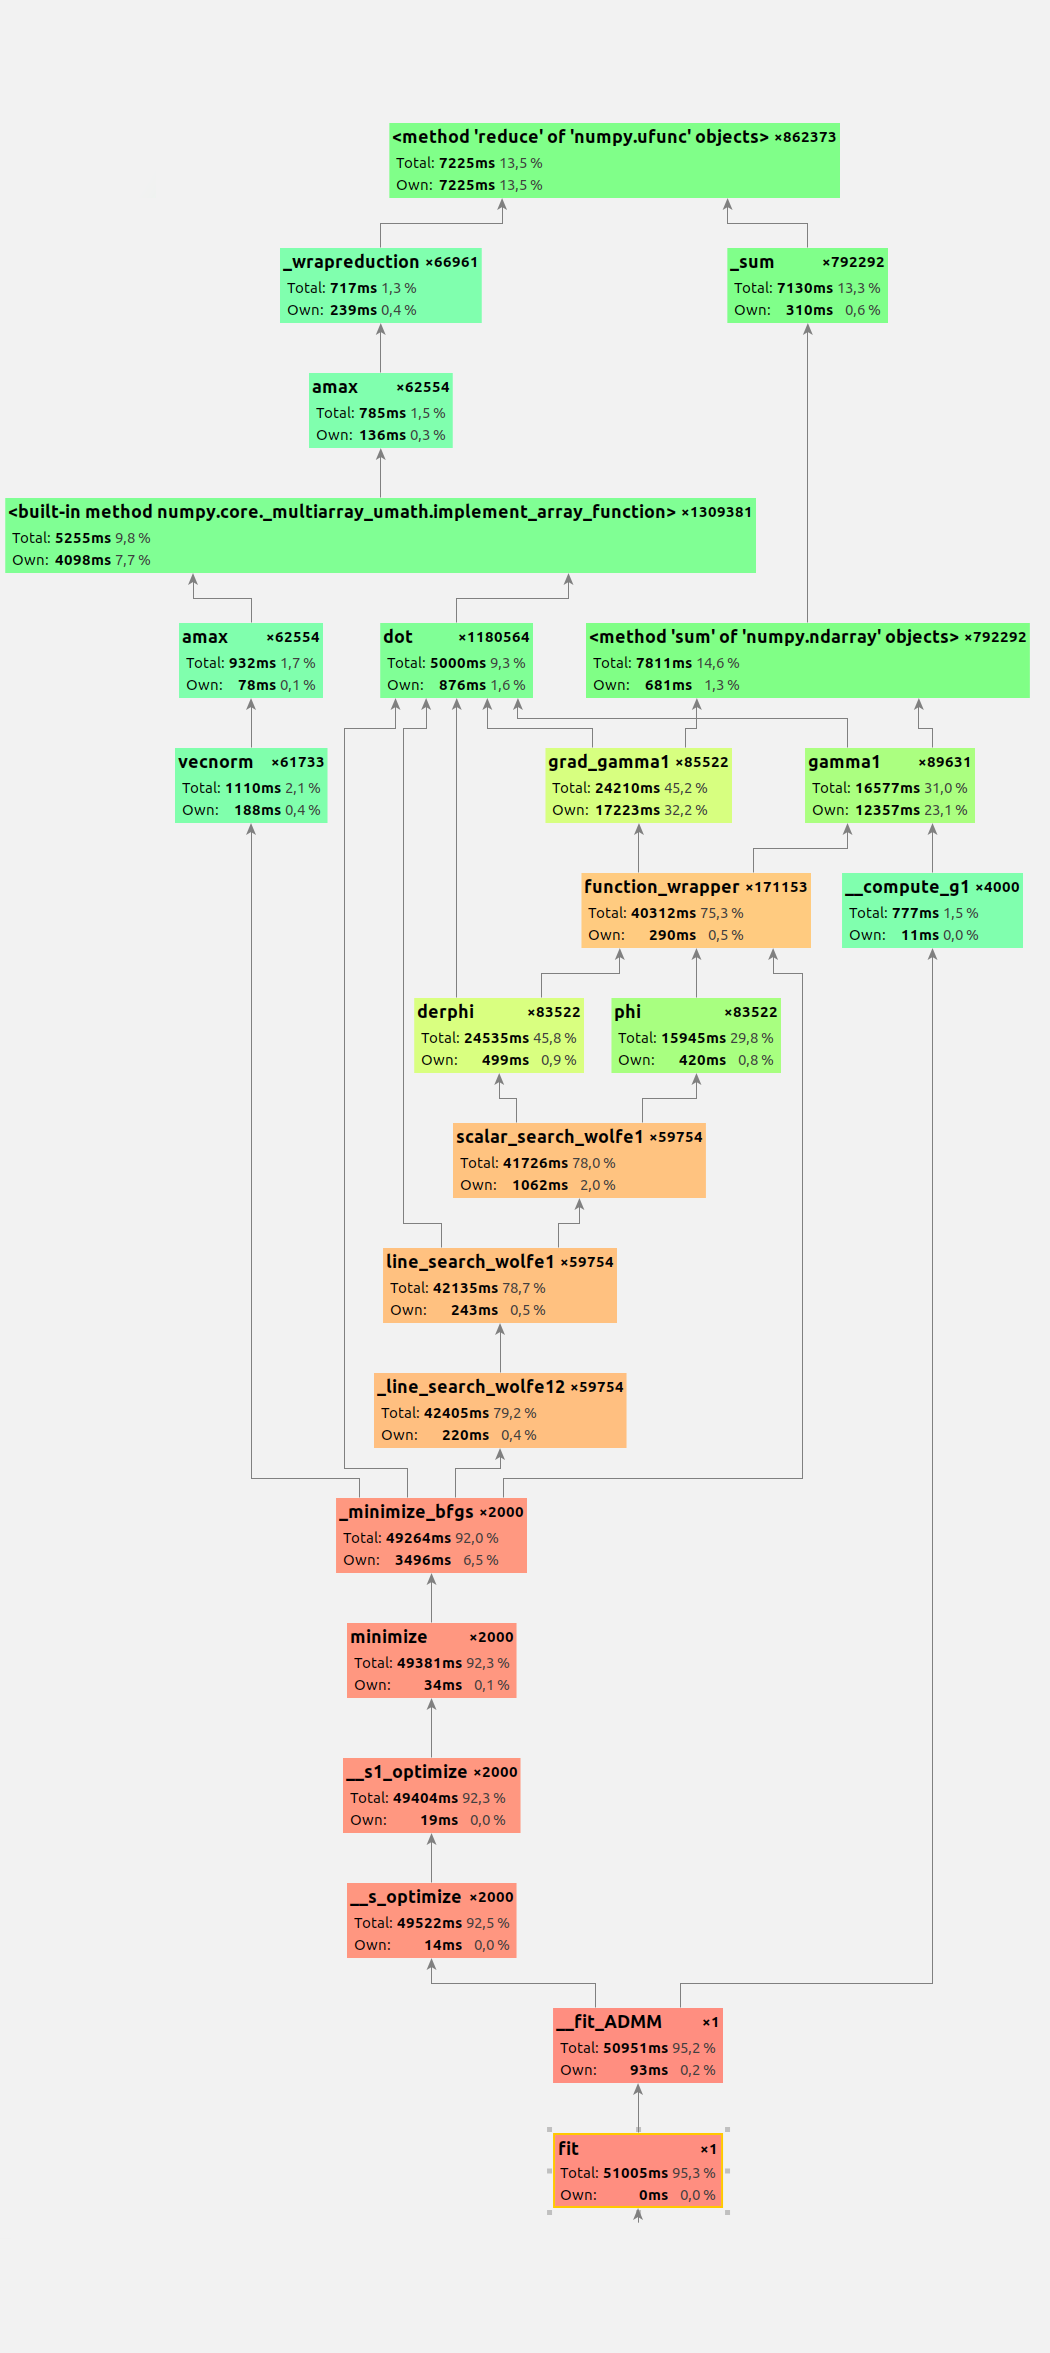
\includegraphics[height=0.88\textheight]{img/profiling2.png}
        \end{center}
    \end{column}
    
    \begin{column}{0.49\textwidth}
        \begin{center}
            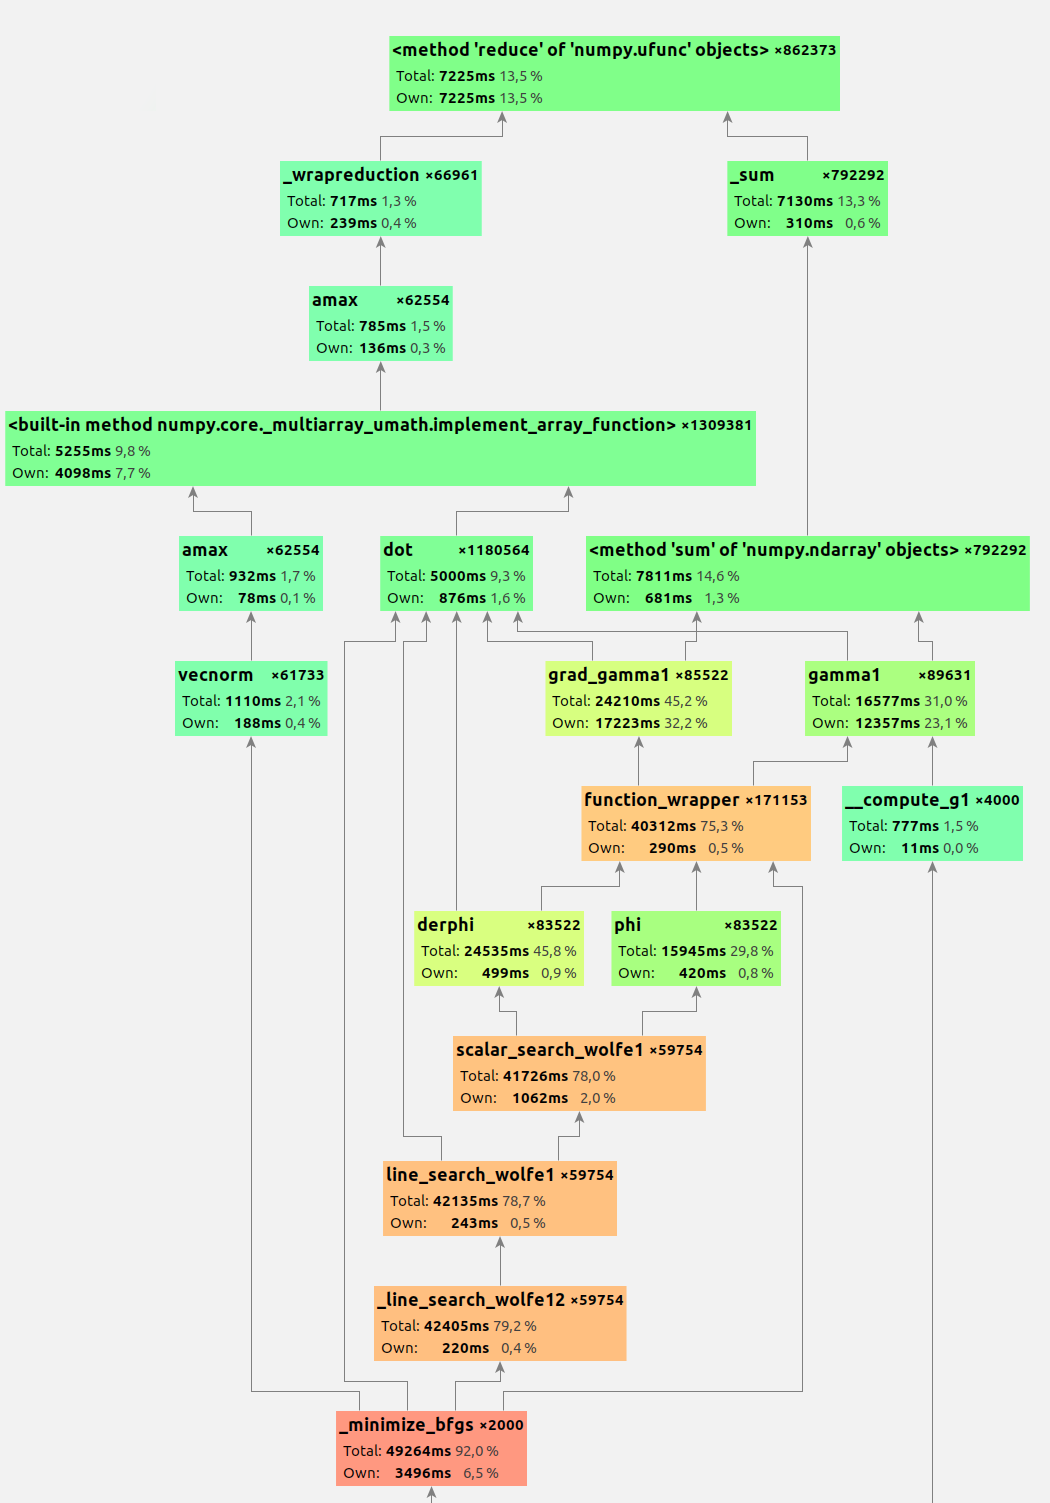
\includegraphics[height=0.88\textheight]{img/profiling3.png}
        \end{center}
    \end{column}
\end{columns}
    
\end{frame}



\begin{frame}{Implementation : semi-supervized learning}

    \begin{block}{Done :}
        \begin{itemize}
            \item $\gamma_1$ and $\nabla(\gamma_1)$ for semi-supervized learning
            \item framework EM (see previous algorithm)
        \end{itemize}
    \end{block}
    \begin{block}{Problem :}
        \begin{itemize}
            \item $\gamma_1$ et $\nabla(\gamma_1)$ must be optimized
            \item Cython implementation in progress
        \end{itemize}
        
    \end{block}
    
\end{frame}

\begin{frame}{$\rho$-update strategy (1/2)}
We can accelerate the training by using the following $\rho$ strategy instead of the Boyd strategy.

\begin{columns}
    \begin{column}{0.48\textwidth}
        \begin{center}
            \large{\textbf{Proposed}}
        \end{center}
        $$
        Q^t = \frac{\left \| pr^t \right \|^2 }{\left \| dr^t \right \|^2 }
        $$
        
        $$
        \rho^{k+1} := \left\{\begin{matrix}
        \rho^t \cdot Q^t & \text{if }  Q^t  > \mu  \text{ or } Q^t < \frac{1}{\mu} \\ 
        \rho^t & \text{otherwise} 
        \end{matrix}\right.
        $$
        
        To be safe , we limit the evolution of $\rho^t$ :
        
        $$
        \frac{1}{\tau^{decr}} \leq Q^t \leq \tau^{incr}
        $$
        
        For example :  $\tau^{decr} = \tau^{incr} = 16, \mu = 4$
    
    \end{column}
    
    \begin{column}{0.48\textwidth}
    \begin{center}
            \large{\textbf{Boyd}}
    \end{center}
    
    $$
    \rho^{k+1} := \left\{\begin{matrix}
    \rho^t \cdot \tau^{incr} & \text{if }  \left \| pr^t \right \|^2   > \mu \cdot \left \| dr^t \right \|^2  \\ 
    \rho^t / \tau^{decr} & \text{if }  \left \| dr^t \right \|^2   > \mu \cdot \left \| pr^t \right \|^2  \\ 
    \rho^t & \text{otherwise} 
    \end{matrix}\right.
    $$
    
    With $\tau^{decr} = \tau^{incr} = 2, \mu = 10$
    
    \end{column}

\end{columns}

\end{frame}

\begin{frame}{$\rho$-update strategy (2/2)}

Results :

\begin{center}
\begin{tabular}{llll}
Dataset & Boyd & Ours & Diff (\%)\\
\hline
Charlotte, C=10, K=30 & 927.4 s & 467.3 s & - 50 \%\\
Charlotte, C=5, K=12 & 183.5 s & 92.7 s & - 49 \%\\
Charlotte, C=2, K=12 & 6.34 s & 3.45 s & - 46 \%\\
Toy, n=2000, C=6, K=16 & 161.8 s & 70.4 s & - 56 \%\\
Formosat-2, n= 10k, C=17, K=30 & 3498.4 s & 1993.3 s & - 43 \%\\
\end{tabular}
\end{center}

\end{frame}

\begin{frame}{Influence of $\gamma_1$ maximum number of iterations}
\begin{columns}
    \begin{column}{0.48\textwidth}
        
        \begin{itemize}
        \item At each iteration of ADMM, we minimize $\gamma_1$ with BFGS algorithm.
        
        \item One of the parameters of this algorithm is the number of iteration.
        
        \item Reducing the maximum number of iterations may improve ADMM speed, while maintaining the same precision at the end of the algorithm.
        \end{itemize}
        
    \end{column}
        \begin{column}{0.48\textwidth}
        
       \begin{center}
        \begin{tabular}{rrr}
        $\gamma_1$ max\textsubscript{iter} & time (s) & ADMM nb\textsubscript{iter}\\
        \hline
        1 & 2.516 & 1169\\
        5 & 2.185 & 501\\
        8 & 2.874 & 466\\
        10 & 3.990 & 546\\
        20 & 7.336 & 555\\
        25 & 8.725 & 555\\
        50 & 9.436 & 555\\
        75 & 9.436 & 555\\
        100 & 9.436 & 555\\
        \end{tabular}
        \end{center}
        
    \end{column}
    See : Boyd, Stephen, et al. "Distributed optimization and statistical learning via the alternating direction method of multipliers." Foundations and Trends® in Machine learning 3.1 (2011): 1-122.
\end{columns}

    
\end{frame}

\begin{frame}{Force constraints at then end of the algorithm}
    \begin{tabular}{cl}  
         \begin{tabular}{c}
           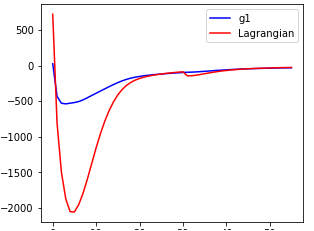
\includegraphics[height=3.5cm, width=4cm]{img/convergence.png}
           \end{tabular}
           & \begin{tabular}{l}
             \parbox{0.5\linewidth}{%  change the parbox width as appropiate
             At the end of the algorithm, the estimated $\mathbf{r^{(t)}}$ is near the optimal value, but does not validate the constraints.
             
             
    }
         \end{tabular}  \\
    
    \end{tabular}
\\

With this almost valid solution, we can find a $\mathbf{r}$ that verify all constraints :

\begin{eqnarray}
      \label{eq:ll:ss}
          \begin{array}{rl}
            \displaystyle{\min_{\mathbf{r}}}
            &\displaystyle{\left \| \mathbf{r}-\mathbf{r^{(t)}} \right\|^2}\\
            
            
               \text{Constraint to} & \mathbf{A}\mathbf{r} = \mathbf{1}\\
              & \mathbf{r} \succcurlyeq 0
          \end{array}
     \end{eqnarray}

\end{frame}


\section{Simulations}

\begin{frame}{Charlotte's Dataset}
    \begin{center}
        
        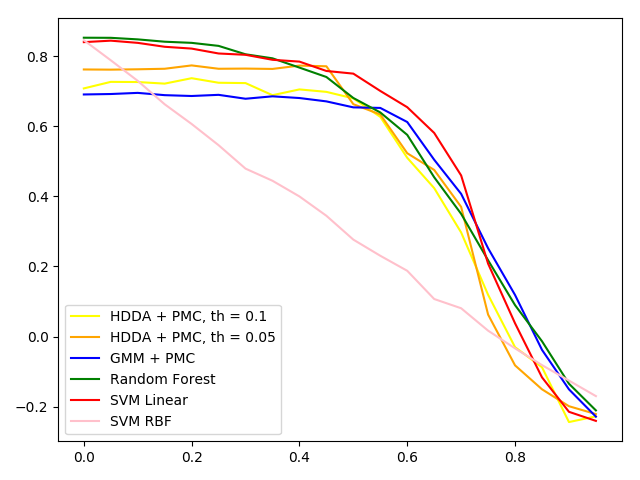
\includegraphics[width=7cm]{img/plot_5classes_hdda_multipleth.png}
        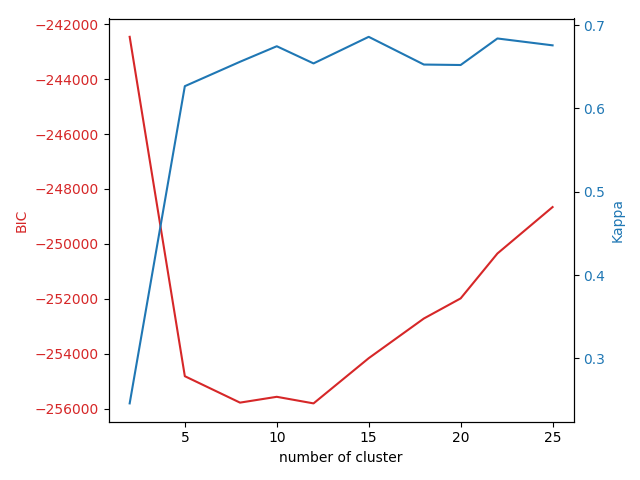
\includegraphics[width=7cm]{img/cluster_bic_5class_gmm.png}
    \end{center}
    
    
    \begin{itemize}
        \item Classification performance depends of clustering quality
        \item BIC can be used to assess clustering quality
    \end{itemize}
    
\end{frame}

\begin{frame}{Formosat-2}
    Mean curves for sunflower :
    \begin{center}
    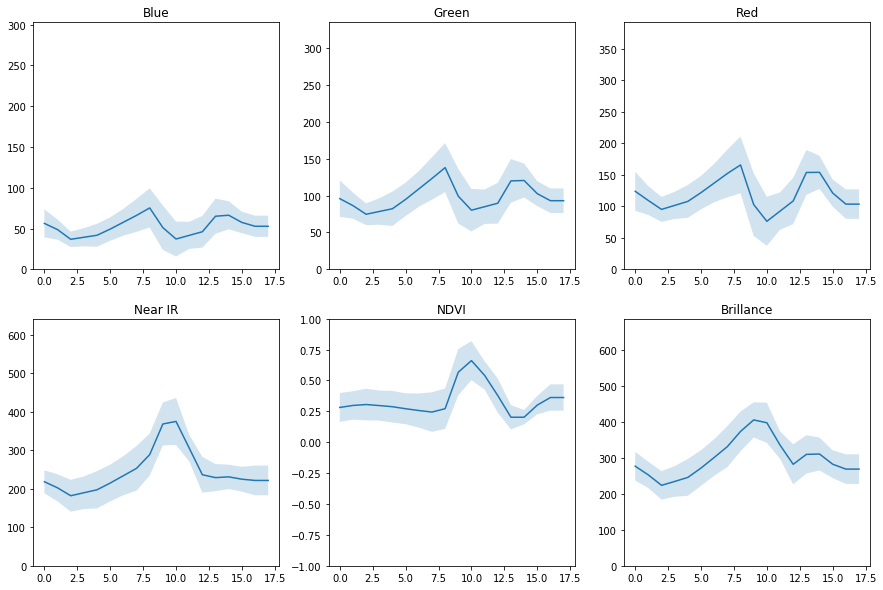
\includegraphics[height=0.8\textheight]{img/tournesol.png}
    \end{center}
    \note[item]{4 bandes spectrales + NDVI + Brillance}
    \note[item]{18 mesures, sur 2013} 
    \note[item]{17 classes}
    \note[item]{gap-filled data}
\end{frame}

\begin{frame}{Formosat-2 : clustering}
    \begin{center}
    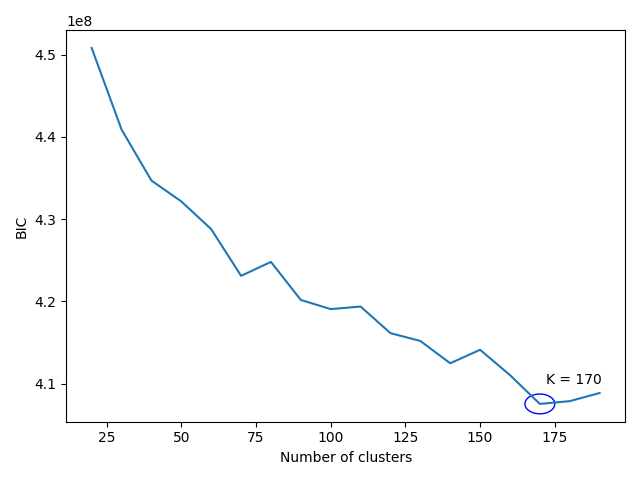
\includegraphics[height=0.7\textheight]{img/clust_formosat.png}\\
    HDDA (impl Python), $tol=10^{-6}$, $th = 0.05$, model = M1
    \end{center}
    
    
\end{frame}

\section{Planning}


\begin{frame}{Journée des doctorants CESBIO, January 2020}
    \begin{itemize}
        \item CESBIO students present their thesis
        \item I will present my thesis (5 min)
        \item Rim ZAIANI, Claire PASCAL and I are conducting this event
    \end{itemize}
\end{frame}

\begin{frame}{Statlearn, 23-27 Mars 2020, Carguese}
    \begin{block}{Lectures}
        \begin{itemize}
            \item  Rianne van den Berg (Google AI, Brian team) : \textbf{Deep generative models}
            \item James Hensman (PROWLER.io): \textbf{Gaussian processes}
            \item Julien Mairal (Inria Grenoble) : \textbf{From kernel methods to deep leaning}
            \item Camille Saumard (Twice.ai): \textbf{Statistical machine learning in a startup}
        \end{itemize}
    \end{block}
    \begin{block}{Organized by :}
        \begin{itemize}
            \item Charles Bouveyron (Université Cote d’Azur \& Inria)
            \item Mathieu Emily (Agrocampus Ouest)
            \item Chloé Friguet (Univ. Bretagne-Sud)
            \item Julien Jacques (Univ. Lyon)
            \item Pierre Latouche (Univ. Paris Descartes)
        \end{itemize}
        
    \end{block}



    
\end{frame}

\begin{frame}{Semi-supervized learning}
\begin{itemize}
    \item Study the weighting between the supervized part and the unsupervized part
    \item Define a correct ratio between the labelled dataset and the unlabelled dataset
    \item Comparison between semi-supervized and supervized learning
\end{itemize}
    
\end{frame}

\begin{frame}{Formosat-2}

    \begin{itemize}
        \item Compare to Random Forest and SVM (linear \& RBF)
    \end{itemize}

    
\end{frame}

\begin{frame}{Biblio}
    \begin{itemize}
        \item Start redaction
        \item Statlearn's poster (March 2020)
        \item Goal : ISPRS2020 (14-20 June 2020)
    \end{itemize}
\end{frame}

%% Le dire à l'oral
% \begin{frame}{Cython implementation}
% Implementation of main functions in Cython, for faster model training.
%     \begin{itemize}
%         \item supervized learning : $\gamma_1$ and $\nabla \gamma_1$
%         \item semi-supervized learning : $\gamma^{semi\-sup}_1$ and $\nabla \gamma^{semi\-sup}_1$
%     \end{itemize}
% \end{frame}







\end{document}
